\begin{figure}
	\center
	\begin{minipage}{0.15\linewidth}
		\center\scriptsize
		Images
	\end{minipage}\hfill
	\begin{minipage}{0.84\linewidth}
	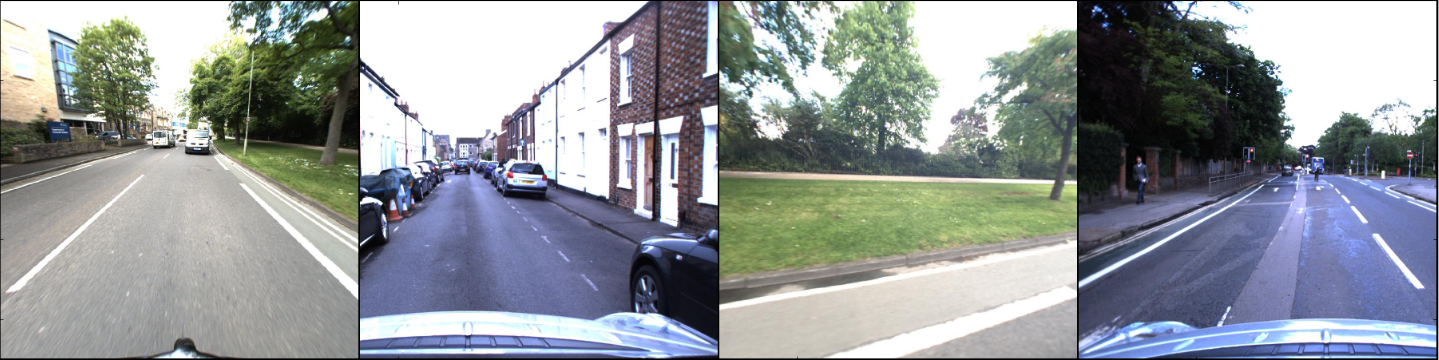
\includegraphics[width=\linewidth]{reflectance/ref_exs/im_1}		
	\end{minipage}
	
	\begin{minipage}{0.15\linewidth}
		\center\scriptsize
		Ground truth reflectance map
	\end{minipage}\hfill
	\begin{minipage}{0.84\linewidth}
	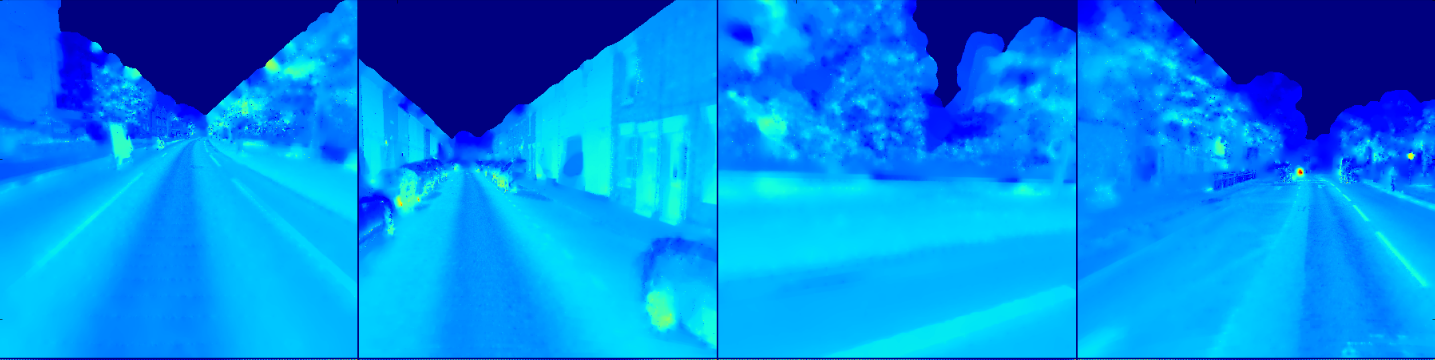
\includegraphics[width=\linewidth]{reflectance/ref_exs/gt_1}	
	\end{minipage}
	
	\begin{minipage}{0.15\linewidth}
		\center\scriptsize		
		Generated reflectance map
	\end{minipage}\hfill
	\begin{minipage}{0.84\linewidth}
	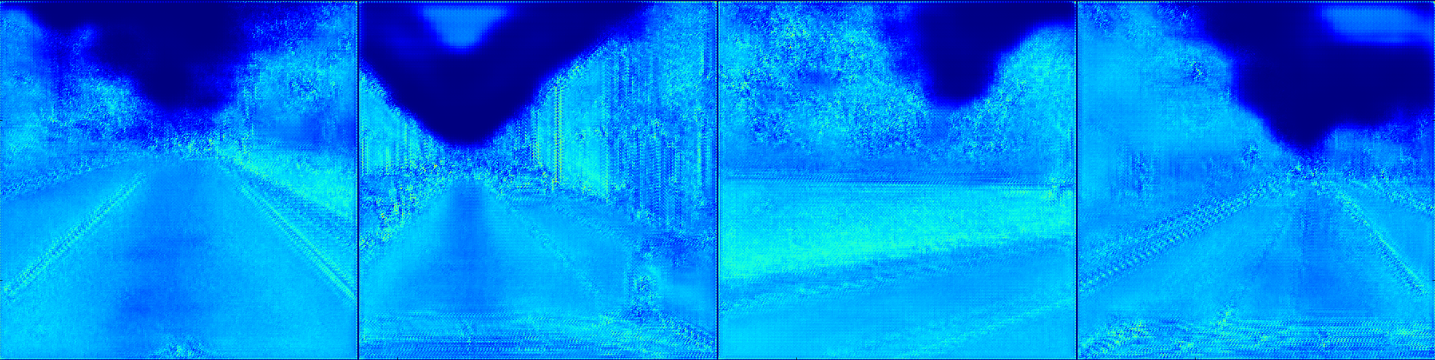
\includegraphics[width=\linewidth]{reflectance/ref_exs/gene_1}	
	\end{minipage}
	
	\caption{\label{fig:ref_examples} \textbf{Examples of dense reflectance map:} the lighter the color, the higher the reflection of the material. Reflectance map highlights reflective areas, like road marking, road sign, vegetation and cars. Figure best viewed in colors.}
\end{figure}